%------------------------------------------------------------------------------
\chapter{Auxiliary Information}
\label{sec:app}
%------------------------------------------------------------------------------

\begin{itemize}
\item MC Samples (Preprod, MC16A)
\item BDT ID studies \texttt{bdt\_tauid}
\item RNN ID studies \texttt{rnn\_tauid}
\item RNN Decay Mode studies \texttt{rnn\_decay\_mode\_classif}
\end{itemize}

\todo[inline]{Tables of layers, i.e.\ keras output for model-summary.}

\section{Auxiliary Figures}

\begin{figure}[htpb]
  \centering
  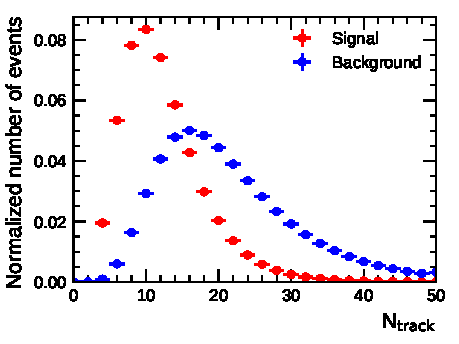
\includegraphics{./figures/rnn/ntrk_3p.pdf}
  \caption{Number of tracks for 3-prong taus}
  \label{fig:total_tracks_3p}
\end{figure}

\begin{figure}[htpb]
  \centering
  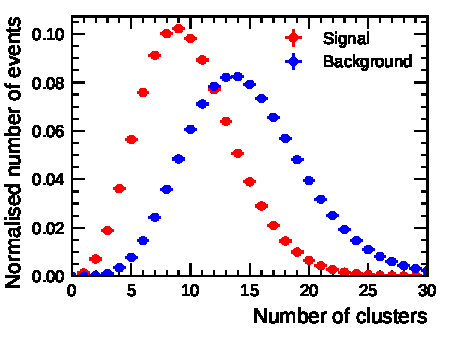
\includegraphics{./figures/rnn/ncls_3p.pdf}
  \caption{Number of clusters for 3-prong taus}
  \label{fig:total_clusters_3p}
\end{figure}

\section{MC Dijet Slices}
Truth $p_\mathrm{T}$ of jet given by anti-$k_\mathrm{T}$ jet algorithm with distance parameter $R=0.6$:
\begin{itemize}
\item[JZ0W] 0 - 20 GeV
\item[JZ1W] 20 - 60 GeV
\item[JZ2W] 60 - 160 GeV
\item[JZ3W] 160 - 400 GeV
\item[JZ4W] 400 - 800 GeV
\item[JZ5W] 800 - 1300 GeV
\item[JZ6W] 1300 - 1800 GeV
\item[JZ7W] 1800 - 2500 GeV
\item[JZ8W] 2500 - 3200 GeV
\end{itemize}

\url{https://svnweb.cern.ch/cern/wsvn/atlasoff/Generators/MC15JobOptions/trunk/share/DSID361xxx/MC15.361021.Pythia8EvtGen_A14NNPDF23LO_jetjet_JZ1W.py}


\url{https://svnweb.cern.ch/cern/wsvn/atlasoff/Generators/MC15JobOptions/trunk/common/Filters/JetFilterAkt6.py}


\url{https://svnweb.cern.ch/cern/wsvn/atlasoff/Generators/MC15JobOptions/trunk/common/Filters/JetFilter_JZX_Fragment.py}

\todo[inline]{Why is JZ0W not used}

\section{Samples}
\label{app:samples}

\subsection{Preproduction Taus}
\label{app:preprod_taus}

\begin{lstlisting}[basicstyle=\small\ttfamily, breaklines=true]
  mc16_13TeV.425200.Pythia8EvtGen_A14NNPDF23LO_Gammatautau_MassWeight.merge.AOD.e5468_s2997_r9064_r8996
\end{lstlisting}

19974000 events

\subsection{MC16A Taus}
\label{app:mc16a_taus}

\begin{lstlisting}[basicstyle=\small\ttfamily, breaklines=true]
  mc16_13TeV.425200.Pythia8EvtGen_A14NNPDF23LO_Gammatautau_MassWeight.merge.AOD.e5468_s3126_r9364_r9315
\end{lstlisting}

29998000 events

\subsection{Preproduction Dijets}
\label{app:preprod_dijets}
For the tau identification studies the momentum slices (JZ1W to JZ6W) are
combined without cross section weighting as the sizes of the generated slices
are chosen such that high momentum candidates are enhanced. A cross section
reweighting would significantly reduce the weights of high momentum slices with
a large number of simulated events compared to the low momentum slices (JZ1W -
JZ2W) where only a small number of events are simulated.

\begin{lstlisting}[basicstyle=\small\ttfamily, breaklines=true]
  mc16_13TeV.361021.Pythia8EvtGen_A14NNPDF23LO_jetjet_JZ1W.merge.AOD.e3569_s2997_r9064_r8996
  mc16_13TeV.361022.Pythia8EvtGen_A14NNPDF23LO_jetjet_JZ2W.merge.AOD.e3668_s2997_r9064_r9078
  mc16_13TeV.361023.Pythia8EvtGen_A14NNPDF23LO_jetjet_JZ3W.merge.AOD.e3668_s2997_r9064_r8996
  mc16_13TeV.361024.Pythia8EvtGen_A14NNPDF23LO_jetjet_JZ4W.merge.AOD.e3668_s2997_r9064_r9078
  mc16_13TeV.361025.Pythia8EvtGen_A14NNPDF23LO_jetjet_JZ5W.merge.AOD.e3668_s2997_r9064_r8996
  mc16_13TeV.361026.Pythia8EvtGen_A14NNPDF23LO_jetjet_JZ6W.merge.AOD.e3569_s2997_r9064_r9078
\end{lstlisting}

JZ1W: 2020000 events \\
JZ2W: 1994000 events \\
JZ3W: 7801500 events \\
JZ4W: 7973500 events \\
JZ5W: 7948500 events \\
JZ6W: 1981000 events \\

\subsection{Upgrade Samples}
Gammatautau (extended layout \cite{itk_layout_slides}):
\begin{lstlisting}[basicstyle=\small\ttfamily, breaklines=true]
  mc15_14TeV.361247.PowhegPythia8EvtGen_AZNLOCTEQ6L1_Ztautau_new.recon.AOD.e4805_s2987_s2999_r8820
  mc15_14TeV.301040.PowhegPythia8EvtGen_AZNLOCTEQ6L1_DYtautau_120M180.recon.AOD.e5323_s2987_s2999_r8820
  mc15_14TeV.301041.PowhegPythia8EvtGen_AZNLOCTEQ6L1_DYtautau_180M250.recon.AOD.e5323_s2987_s2999_r8820
  mc15_14TeV.301042.PowhegPythia8EvtGen_AZNLOCTEQ6L1_DYtautau_250M400.recon.AOD.e5323_s2987_s2999_r8820
  mc15_14TeV.301043.PowhegPythia8EvtGen_AZNLOCTEQ6L1_DYtautau_400M600.recon.AOD.e5323_s2987_s2999_r8820
  mc15_14TeV.301044.PowhegPythia8EvtGen_AZNLOCTEQ6L1_DYtautau_600M800.recon.AOD.e5323_s2987_s2999_r8820
  mc15_14TeV.301045.PowhegPythia8EvtGen_AZNLOCTEQ6L1_DYtautau_800M1000.recon.AOD.e5323_s2987_s2999_r8820
  mc15_14TeV.301046.PowhegPythia8EvtGen_AZNLOCTEQ6L1_DYtautau_1000M1250.recon.AOD.e5323_s2987_s2999_r8820
  mc15_14TeV.301047.PowhegPythia8EvtGen_AZNLOCTEQ6L1_DYtautau_1250M1500.recon.AOD.e5323_s2987_s2999_r8820
  mc15_14TeV.301048.PowhegPythia8EvtGen_AZNLOCTEQ6L1_DYtautau_1500M1750.recon.AOD.e5323_s2987_s2999_r8820
  mc15_14TeV.301049.PowhegPythia8EvtGen_AZNLOCTEQ6L1_DYtautau_1750M2000.recon.AOD.e5323_s2987_s2999_r8820
  mc15_14TeV.301050.PowhegPythia8EvtGen_AZNLOCTEQ6L1_DYtautau_2000M2250.recon.AOD.e5323_s2987_s2999_r8820
  mc15_14TeV.301051.PowhegPythia8EvtGen_AZNLOCTEQ6L1_DYtautau_2250M2500.recon.AOD.e5323_s2987_s2999_r8820
  mc15_14TeV.301052.PowhegPythia8EvtGen_AZNLOCTEQ6L1_DYtautau_2500M2750.recon.AOD.e5323_s2987_s2999_r8820
  mc15_14TeV.301053.PowhegPythia8EvtGen_AZNLOCTEQ6L1_DYtautau_2750M3000.recon.AOD.e5323_s2987_s2999_r8820
  mc15_14TeV.301054.PowhegPythia8EvtGen_AZNLOCTEQ6L1_DYtautau_3000M3500.recon.AOD.e5323_s2987_s2999_r8820
  mc15_14TeV.301055.PowhegPythia8EvtGen_AZNLOCTEQ6L1_DYtautau_3500M4000.recon.AOD.e5323_s2987_s2999_r8820
  mc15_14TeV.301056.PowhegPythia8EvtGen_AZNLOCTEQ6L1_DYtautau_4000M4500.recon.AOD.e5323_s2987_s2999_r8820
  mc15_14TeV.301057.PowhegPythia8EvtGen_AZNLOCTEQ6L1_DYtautau_4500M5000.recon.AOD.e5323_s2987_s2999_r8820
  mc15_14TeV.301058.PowhegPythia8EvtGen_AZNLOCTEQ6L1_DYtautau_5000M.recon.AOD.e5323_s2987_s2999_r8820
\end{lstlisting}

Ztautau: 300000
120M180: 150000\\
180M250: 150000\\
250M400: 150000\\
400M600: 147300\\
600M800: 50000\\
800M1000: 50000\\
1000M1250: 50000\\
1250M1500: 50000\\
1500M1750: 49900\\
1750M2000: 50000\\
2000M2250: 49900\\
2250M2500: 50000\\
2500M2750: 50000\\
2750M3000: 50000\\
3000M3500: 50000\\
3500M4000: 50000\\
4000M4500: 50000\\
4500M5000: 50000\\
5000M: 49900

Dijets (extended layout):
\begin{lstlisting}[basicstyle=\small\ttfamily, breaklines=true]
  mc15_14TeV.147910.Pythia8_AU2CT10_jetjet_JZ0W.recon.AOD.e2403_s2987_s2999_r8820
  mc15_14TeV.147911.Pythia8_AU2CT10_jetjet_JZ1W.recon.AOD.e2403_s2987_s2999_r8820
  mc15_14TeV.147912.Pythia8_AU2CT10_jetjet_JZ2W.recon.AOD.e2403_s2987_s2999_r8820
  mc15_14TeV.147913.Pythia8_AU2CT10_jetjet_JZ3W.recon.AOD.e2403_s2987_s2999_r8820
  mc15_14TeV.147914.Pythia8_AU2CT10_jetjet_JZ4W.recon.AOD.e2403_s2987_s2999_r8820
  mc15_14TeV.147915.Pythia8_AU2CT10_jetjet_JZ5W.recon.AOD.e2403_s2987_s2999_r8820
  mc15_14TeV.147916.Pythia8_AU2CT10_jetjet_JZ6W.recon.AOD.e2403_s2987_s2999_r8820
  mc15_14TeV.147917.Pythia8_AU2CT10_jetjet_JZ7W.recon.AOD.e2403_s2987_s2999_r8820
\end{lstlisting}

JZ0W:999500\\
JZ1W:962300\\
JZ2W:999500\\
JZ3W:985400\\
JZ4W:50000\\
JZ5W:49650\\
JZ6W:50000\\
JZ7W:50000


\clearpage
\section{Tau-ID Variables}
\label{app:tauid_vars}

\subsection{1-prong}
\begin{figure}[!ht]
  \begin{subfigure}{0.5\textwidth}
    \centering
    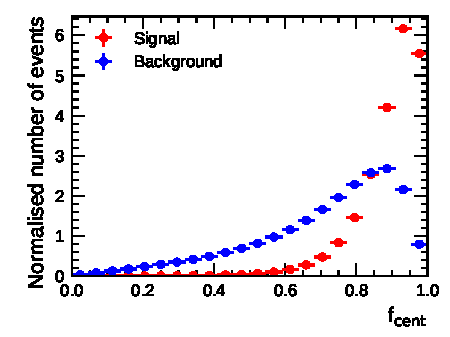
\includegraphics{./figures/baseline_bdt_vars/1p/centFrac.pdf}
  \end{subfigure}%
  \begin{subfigure}{0.5\textwidth}
    \centering
    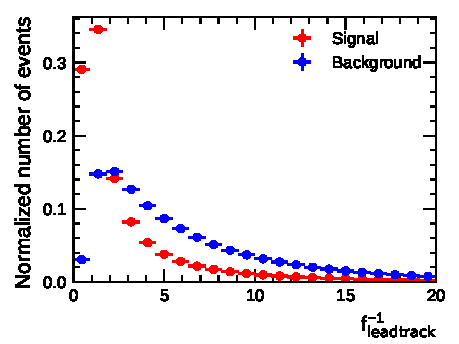
\includegraphics{./figures/baseline_bdt_vars/1p/etOverPtLeadTrk.pdf}
  \end{subfigure}
  \begin{subfigure}{0.5\textwidth}
    \centering
    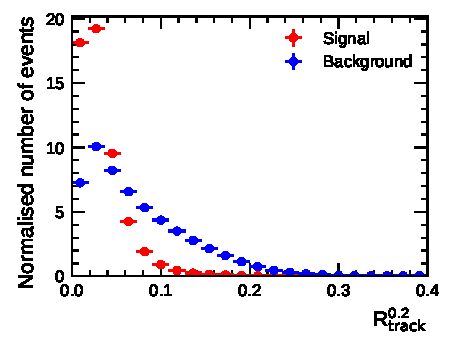
\includegraphics{./figures/baseline_bdt_vars/1p/innerTrkAvgDist.pdf}
  \end{subfigure}%
  \begin{subfigure}{0.5\textwidth}
    \centering
    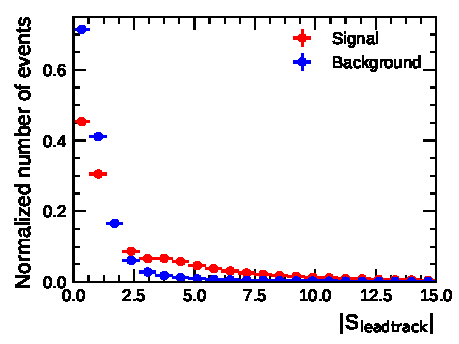
\includegraphics{./figures/baseline_bdt_vars/1p/absipSigLeadTrk.pdf}
  \end{subfigure}
  \begin{subfigure}{0.5\textwidth}
    \centering
    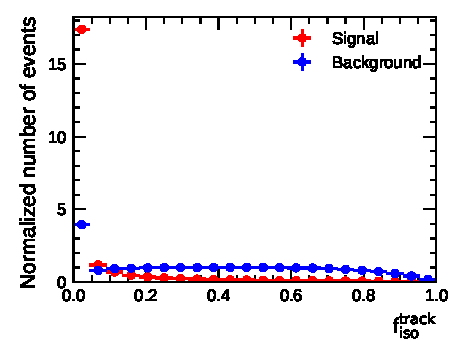
\includegraphics{./figures/baseline_bdt_vars/1p/SumPtTrkFrac.pdf}
  \end{subfigure}%
  \begin{subfigure}{0.5\textwidth}
    \centering
    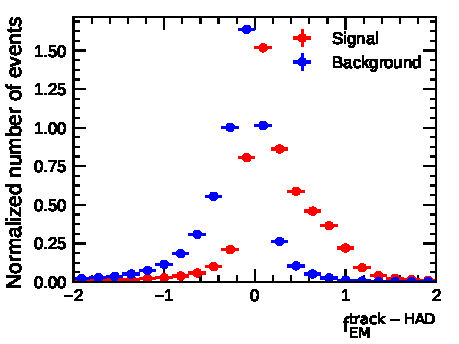
\includegraphics{./figures/baseline_bdt_vars/1p/ChPiEMEOverCaloEME.pdf}
  \end{subfigure}
  \caption{Variables used in Tau-ID BDT. \mytodo{Rename innerTrkAvgDist x-label}}
  \label{fig:bdt_vars_1p_overlays}
\end{figure}

\begin{figure}[!ht]\ContinuedFloat
  \begin{subfigure}{0.5\textwidth}
    \centering
    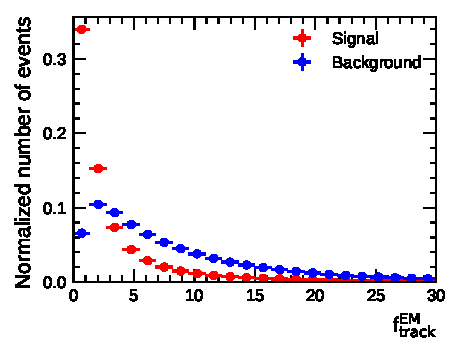
\includegraphics{./figures/baseline_bdt_vars/1p/EMPOverTrkSysP.pdf}
  \end{subfigure}%
  \begin{subfigure}{0.5\textwidth}
    \centering
    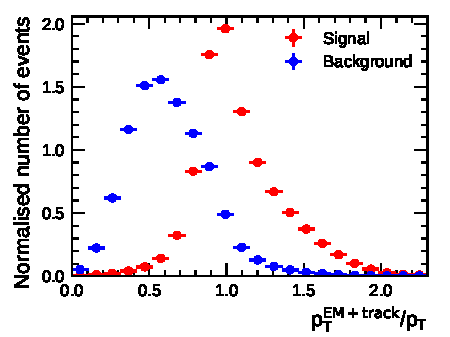
\includegraphics{./figures/baseline_bdt_vars/1p/ptRatioEflowApprox.pdf}
  \end{subfigure}
  \begin{subfigure}{0.5\textwidth}
    \centering
    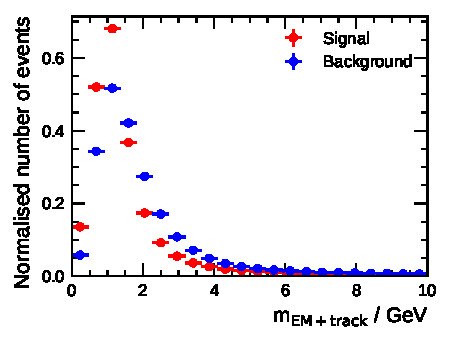
\includegraphics{./figures/baseline_bdt_vars/1p/mEflowApprox.pdf}
  \end{subfigure}
  \caption[]{Variables used in Tau-ID BDT}
\end{figure}

\clearpage
\subsection{3-prong}

\begin{figure}[!ht]
  \begin{subfigure}{0.5\textwidth}
    \centering
    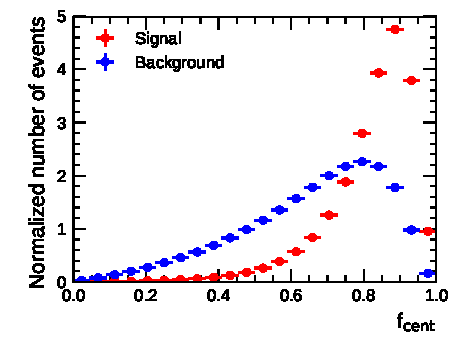
\includegraphics{./figures/baseline_bdt_vars/3p/centFrac.pdf}
  \end{subfigure}%
  \begin{subfigure}{0.5\textwidth}
    \centering
    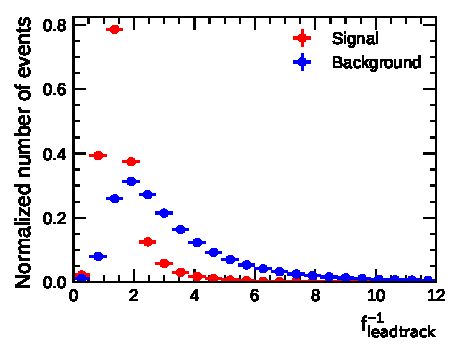
\includegraphics{./figures/baseline_bdt_vars/3p/etOverPtLeadTrk.pdf}
  \end{subfigure}
  \begin{subfigure}{0.5\textwidth}
    \centering
    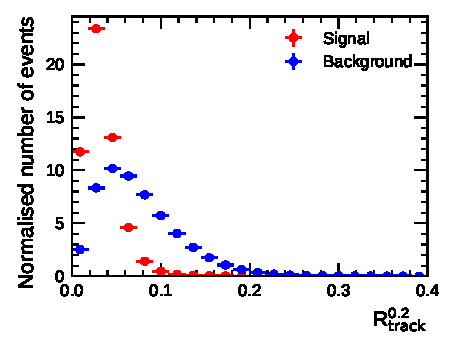
\includegraphics{./figures/baseline_bdt_vars/3p/innerTrkAvgDist.pdf}
  \end{subfigure}%
  \begin{subfigure}{0.5\textwidth}
    \centering
    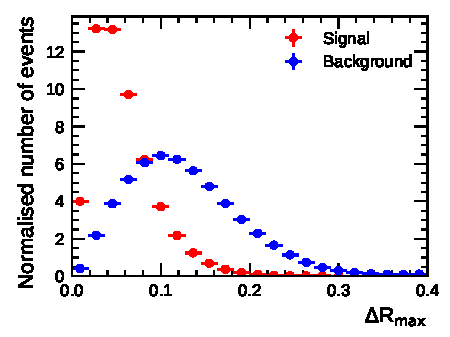
\includegraphics{./figures/baseline_bdt_vars/3p/dRmax.pdf}
  \end{subfigure}
  \begin{subfigure}{0.5\textwidth}
    \centering
    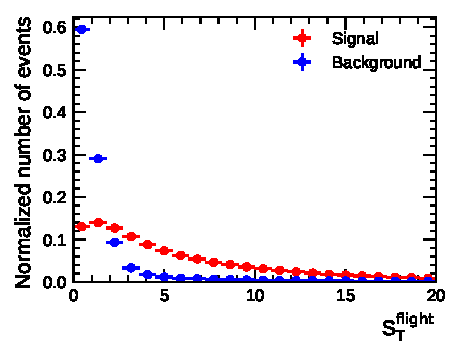
\includegraphics{./figures/baseline_bdt_vars/3p/trFlightPathSig.pdf}
  \end{subfigure}%
  \begin{subfigure}{0.5\textwidth}
    \centering
    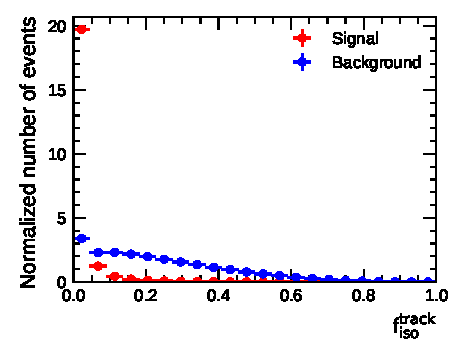
\includegraphics{./figures/baseline_bdt_vars/3p/SumPtTrkFrac.pdf}
  \end{subfigure}%
  \caption{Variables used in Tau-ID BDT\mytodo{rename innerTrkAvgDist x-label}}
  \label{fig:bdt_vars_3p_overlays}
\end{figure}

\begin{figure}[!ht]\ContinuedFloat
  \begin{subfigure}{0.5\textwidth}
    \centering
    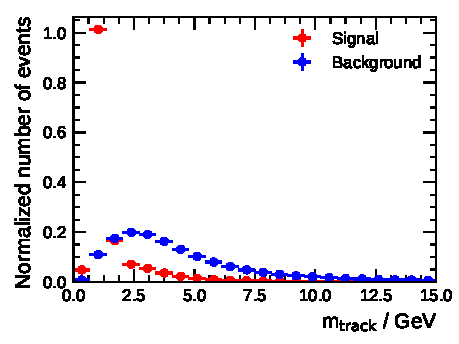
\includegraphics{./figures/baseline_bdt_vars/3p/massTrkSys.pdf}
  \end{subfigure}%
  \begin{subfigure}{0.5\textwidth}
    \centering
    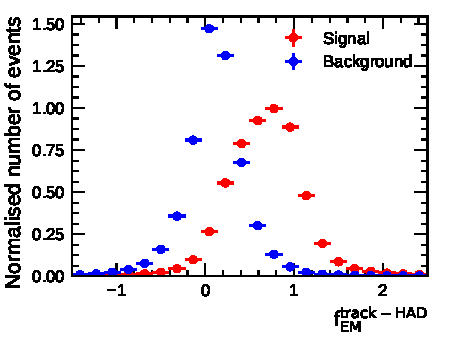
\includegraphics{./figures/baseline_bdt_vars/3p/ChPiEMEOverCaloEME.pdf}
  \end{subfigure}
  \begin{subfigure}{0.5\textwidth}
    \centering
    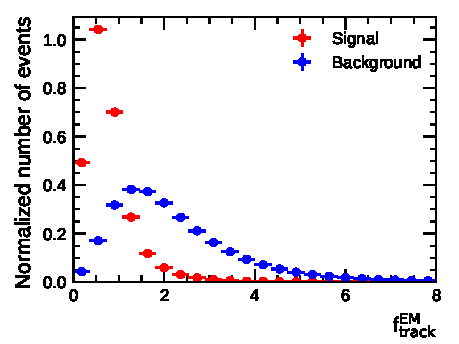
\includegraphics{./figures/baseline_bdt_vars/3p/EMPOverTrkSysP.pdf}
  \end{subfigure}%
  \begin{subfigure}{0.5\textwidth}
    \centering
    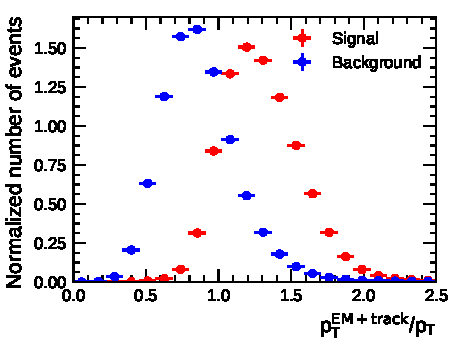
\includegraphics{./figures/baseline_bdt_vars/3p/ptRatioEflowApprox.pdf}
  \end{subfigure}
  \begin{subfigure}{0.5\textwidth}
    \centering
    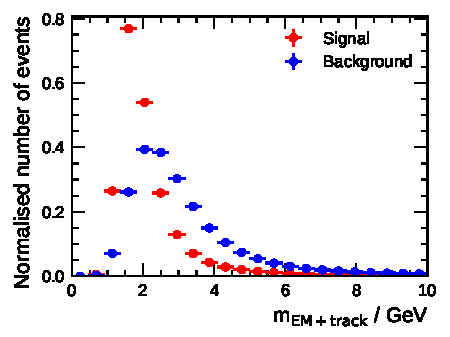
\includegraphics{./figures/baseline_bdt_vars/3p/mEflowApprox.pdf}
  \end{subfigure}
  \caption[]{Variables used in Tau-ID BDT}
\end{figure}

\clearpage
\section{Transformed Variables}
\label{app:variable_transforms}

\begin{table}[htb]
  \centering
  \begin{tabular}{ll}
  \toprule
  Variable & Transformation \\
  \midrule
  \smash{$f_\text{cent}$} & \smash{$\min(x, 1)$} \\
  \smash{$f_\text{leadtrack}^{-1}$} & \smash{$\log(\max(0.1, x))$} \\
  \smash{$R_\text{track}$} & -- \\
  \smash{$\Delta R_\text{max}$} & -- \\
  \smash{$| S_\text{leadtrack} |$} & \smash{$\min(x, 30)$} \\
  \smash{$S_\text{T}^\text{flight}$} & \smash{$\log(\max(0.01, x))$} \\
  \bottomrule
\end{tabular}\hspace*{2em}
\begin{tabular}{ll}
  \toprule
  Variable & Transformation \\
  \midrule
  \smash{$f_\text{iso}^\text{track}$} & \smash{$\log\left(x + 10^{-4}\right)$} \\
  \smash{$f_\text{EM}^\text{track-HAD}$} & \smash{$\max(-4, \min(x, 5))$} \\
  \smash{$f_\text{track}^\text{EM}$} & \smash{$\log\left(\max\left(10^{-3}, x\right)\right)$} \\
  \smash{$p_\text{T}^\text{EM+track} / p_\text{T}$} & \smash{$\min(x, 4)$} \\
  \smash{$m_\text{EM+track}$} & \smash{$\log\left(\max(140, x / \si{\MeV})\right)$} \\
  \smash{$m_\text{track}$} & \smash{$\log\left(\max(140, x / \si{MeV})\right)$} \\
  \bottomrule
\end{tabular}


%%% Local Variables:
%%% mode: latex
%%% TeX-master: "../mythesis"
%%% End:

  \caption{Transformation applied to the input variables}
\end{table}

\clearpage
\section{TMVA-BDT Configurations}
\label{app:tmva_config}

\noindent\textbf{Common for all configurations:}\\[0.3em]
\begin{tabular}{ll}
  \texttt{NegWeightTreatment} & \texttt{IgnoreNegWeightsInTraining} \\
  \texttt{PruneMethod} & \texttt{NoPruning} \\
  \texttt{SeparationType} & \texttt{GiniIndex} \\
  \texttt{UseYesNoLeaf} & \texttt{False} \\
  \texttt{nCuts} & 200
\end{tabular}

\vfill

\noindent\textbf{Old configuration:}\\[0.3em]
\begin{tabular}{ll}
  \texttt{BoostType} & \texttt{AdaBoost} \\
  \texttt{AdaBoostBeta} & 0.2 \\
  \texttt{NTrees} & 100 \\
  \texttt{MaxDepth} & 8 \\
  \texttt{MinNodeSize} & 0.1 \\
\end{tabular}

\vfill

\noindent\textbf{1-prong (Overtrained):}\\[0.3em]
\begin{tabular}{ll}
  \texttt{BoostType} & \texttt{Grad} \\
  \texttt{Shrinkage} & 0.05 \\
  \texttt{NTrees} & 800 \\
  \texttt{MaxDepth} & 16 \\
  \texttt{MinNodeSize} & 0.01 \\
\end{tabular}

\vfill

\noindent\textbf{1-prong (cool):}\\[0.3em]
\begin{tabular}{ll}
  \texttt{BoostType} & \texttt{Grad} \\
  \texttt{Shrinkage} & 0.1 \\
  \texttt{NTrees} & 400 \\
  \texttt{UseBaggedBoost} & \texttt{True} \\
  \texttt{BaggedSampleFraction} & 0.5 \\
  \texttt{MaxDepth} & 8 \\
  \texttt{MinNodeSize} & 0.1 \\
\end{tabular}

\vfill

\noindent\textbf{3-prong (Overtrained):}\\[0.3em]
\begin{tabular}{ll}
  \texttt{BoostType} & \texttt{Grad} \\
  \texttt{Shrinkage} & 0.1 \\
  \texttt{NTrees} & 800 \\
  \texttt{MaxDepth} & 16 \\
  \texttt{MinNodeSize} & 0.01 \\
\end{tabular}

\vfill

\noindent\textbf{3-prong (cool):}\\[0.3em]
\begin{tabular}{ll}
  \texttt{BoostType} & \texttt{Grad} \\
  \texttt{Shrinkage} & 0.4 \\
  \texttt{NTrees} & 800 \\
  \texttt{MaxDepth} & 6 \\
  \texttt{MinNodeSize} & 0.1 \\
\end{tabular}

\clearpage
\section{BDT Stuff}
\label{app:bdt_stuff}

\begin{figure}[ht]
  \begin{subfigure}[t]{0.48\textwidth}
    \centering
    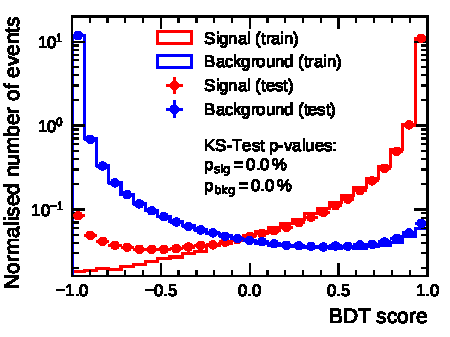
\includegraphics{./figures/bdt_perf/scores/grid_3p0317.pdf}
    \subcaption{BDT A (3-prong)}
  \end{subfigure}
  \begin{subfigure}[t]{0.48\textwidth}
    \centering
    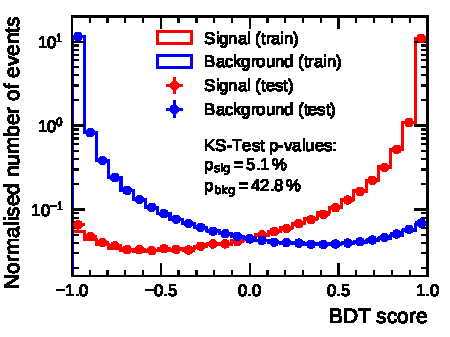
\includegraphics{./figures/bdt_perf/scores/grid_3p0327.pdf}
    \subcaption{BDT B (3-prong)}
  \end{subfigure}
  \caption{Distributions of the 3-prong tau identification BDT score for the
    training and testing sample for both signal and background.}
  \label{fig:bdt_ks5_scores}
\end{figure}

\begin{figure}[ht]
  \begin{subfigure}[t]{0.48\textwidth}
    \centering
    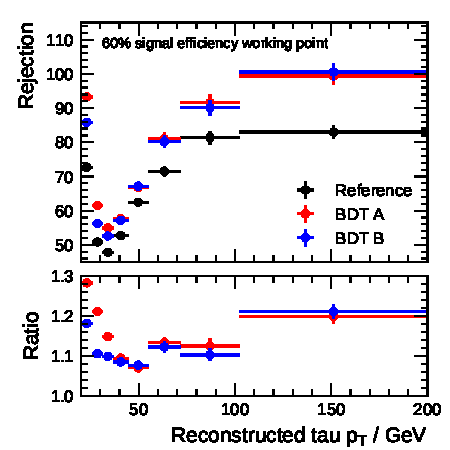
\includegraphics{./figures/bdt_perf/rejection/post_gridsearch_1p/rejection_tight.pdf}
    \subcaption{1-prong (tight)}
  \end{subfigure}\hfill
  \begin{subfigure}[t]{0.48\textwidth}
    \centering
    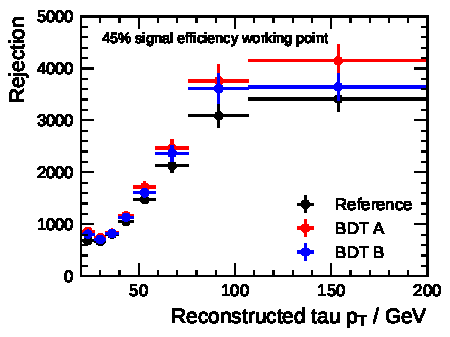
\includegraphics{./figures/bdt_perf/rejection/post_gridsearch_3p/rejection_tight.pdf}
    \subcaption{3-prong (tight)}
  \end{subfigure}
  \caption{Working points (BDT A) \mytodo{Larger pt range in appendix}.
    \mytodo{Ratio is bootstrapped due to highly correlated errors}}
\end{figure}


\clearpage
\section{Decay Mode Classification using Recurrent Neural Networks}
\subsection{Baseline Probabilities}
\label{app:baseline_probabilities}

\begin{figure}[!ht]
  \begin{subfigure}{0.48\textwidth}
    \centering
    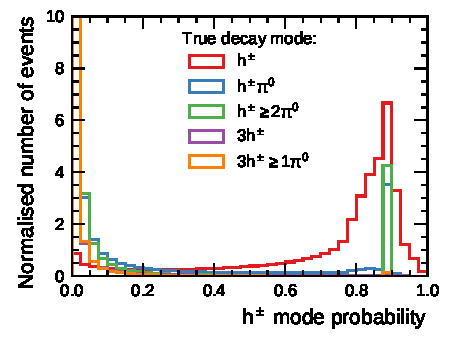
\includegraphics{./figures/decay_mode_classification/mode_proba_baseline_ptcut_1_5/proba_1p0n.pdf}
  \end{subfigure}\hfill
  \begin{subfigure}{0.48\textwidth}
    \centering
    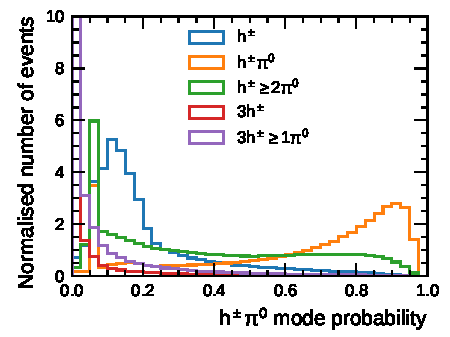
\includegraphics{./figures/decay_mode_classification/mode_proba_baseline_ptcut_1_5/proba_1p1n.pdf}
  \end{subfigure}
  \begin{subfigure}{0.48\textwidth}
    \centering
    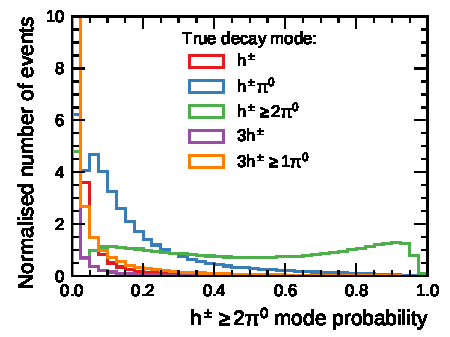
\includegraphics{./figures/decay_mode_classification/mode_proba_baseline_ptcut_1_5/proba_1pXn.pdf}
  \end{subfigure}\hfill
  \begin{subfigure}{0.48\textwidth}
    \centering
    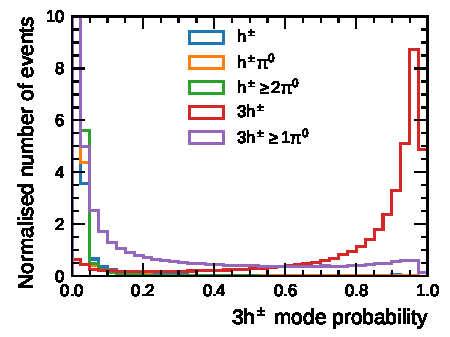
\includegraphics{./figures/decay_mode_classification/mode_proba_baseline_ptcut_1_5/proba_3p0n.pdf}
  \end{subfigure}
  \begin{subfigure}{0.48\textwidth}
    \centering
    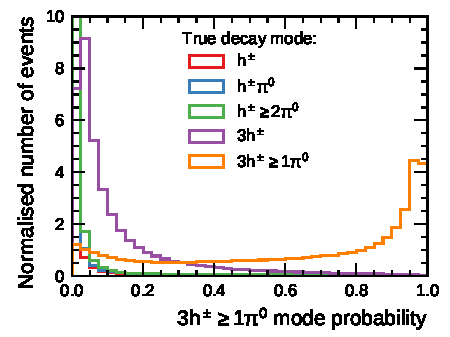
\includegraphics{./figures/decay_mode_classification/mode_proba_baseline_ptcut_1_5/proba_3pXn.pdf}
  \end{subfigure}%

  \caption{Multi-class probabilities for the Baseline RNN}
  \label{fig:rnn_multiclass_proba_baseline}
\end{figure}

\clearpage
\subsection{Combined Probabilities}
\label{app:combined_probabilities}

\begin{figure}[!ht]
  \begin{subfigure}{0.48\textwidth}
    \centering
    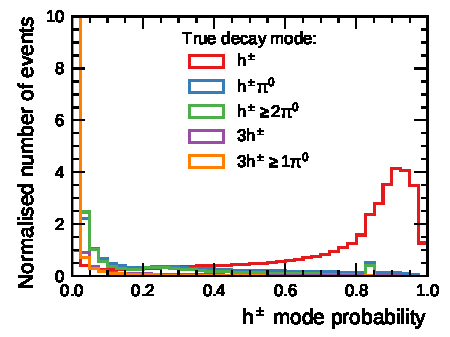
\includegraphics{./figures/decay_mode_classification/combined_proba/proba_1p0n.pdf}
  \end{subfigure}\hfill
  \begin{subfigure}{0.48\textwidth}
    \centering
    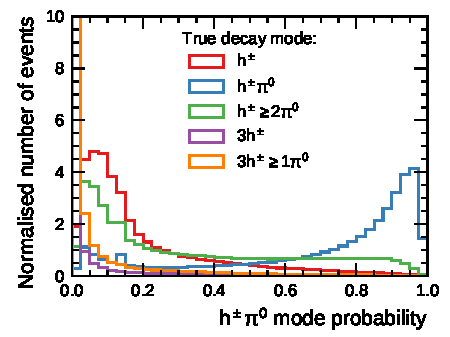
\includegraphics{./figures/decay_mode_classification/combined_proba/proba_1p1n.pdf}
  \end{subfigure}
  \begin{subfigure}{0.48\textwidth}
    \centering
    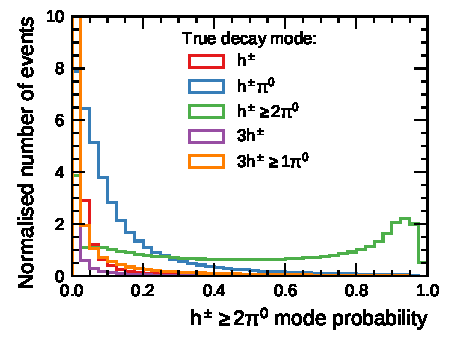
\includegraphics{./figures/decay_mode_classification/combined_proba/proba_1pXn.pdf}
  \end{subfigure}\hfill
  \begin{subfigure}{0.48\textwidth}
    \centering
    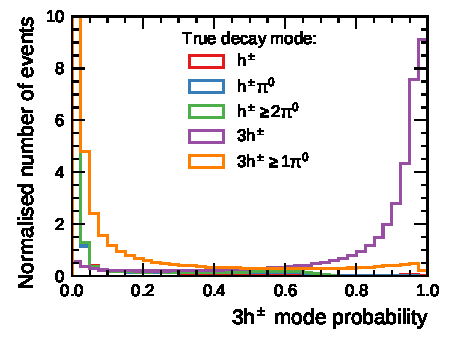
\includegraphics{./figures/decay_mode_classification/combined_proba/proba_3p0n.pdf}
  \end{subfigure}
  \begin{subfigure}{0.48\textwidth}
    \centering
    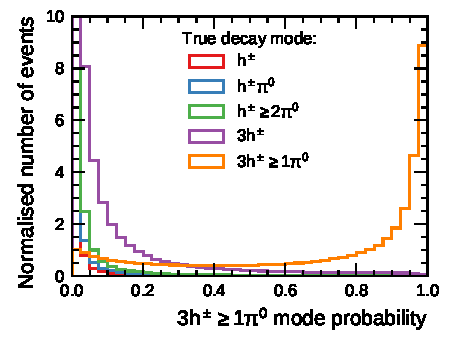
\includegraphics{./figures/decay_mode_classification/combined_proba/proba_3pXn.pdf}
  \end{subfigure}%

  \caption{Multi-class probabilities for the Combined RNN}
  \label{fig:rnn_multiclass_proba_combined}
\end{figure}

\clearpage
\section{Grid Search: 3-Prong}
\label{app:grid_search_3p}

\begin{figure}[htbp]
  \begin{subfigure}[t]{0.48\textwidth}
    \centering
    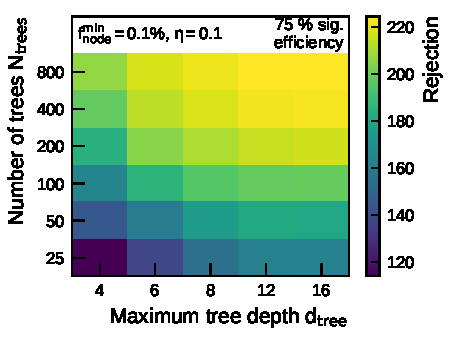
\includegraphics{./figures/bdt_perf/gridsearch_3p/scan_MaxDepth_NTrees.pdf}
    \subcaption{}
  \end{subfigure}\hfill
  \begin{subfigure}[t]{0.48\textwidth}
    \centering
    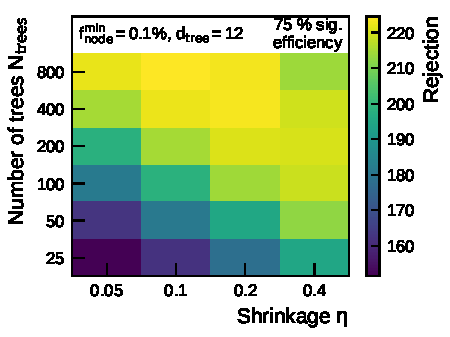
\includegraphics{./figures/bdt_perf/gridsearch_3p/scan_Shrinkage_NTrees.pdf}
    \subcaption{}
  \end{subfigure}
  \begin{subfigure}[t]{0.48\textwidth}
    \centering
    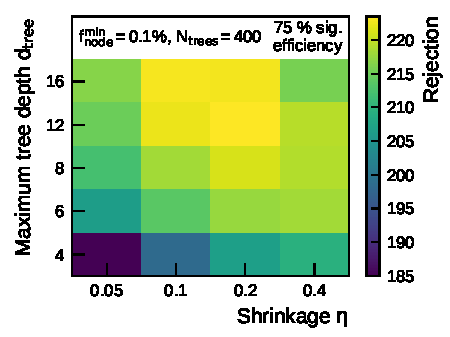
\includegraphics{./figures/bdt_perf/gridsearch_3p/scan_Shrinkage_MaxDepth.pdf}
    \subcaption{}
  \end{subfigure}\hfill
  \begin{subfigure}[t]{0.48\textwidth}
    \centering
    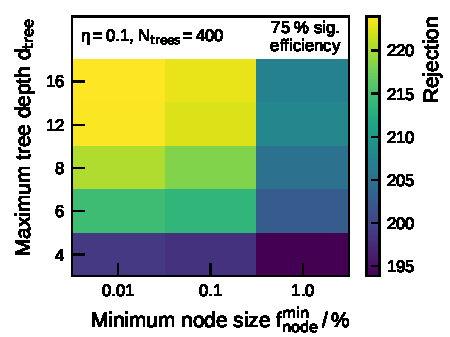
\includegraphics{./figures/bdt_perf/gridsearch_3p/scan_MinNodeSize_MaxDepth.pdf}
    \subcaption{}
  \end{subfigure}
  \caption{Background rejection at \SI{60}{\percent} signal efficiency as a
    function of the BDT hyperparameters. Bagged boosting with a subsample
    fraction~$f_\text{bag} = \SI{50}{\percent}$ is used and the remaining
    parameters are fixed such that the 'best' BDT is contained within the
    plots.}
  \todo[inline]{Better word for 'best' as it is not the best BDT}
  \label{fig:hyperparameter_scan_3p}
\end{figure}

\clearpage
\section{BDT: Recursive Feature Elimination}

\begin{figure}[htb]
  \centering
  \begin{subfigure}[t]{0.33\textwidth}
    \centering
    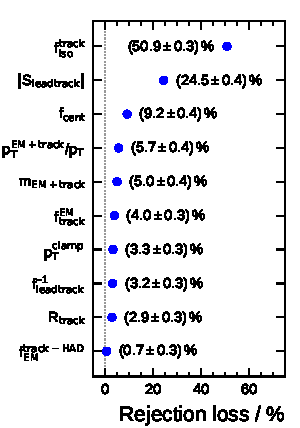
\includegraphics{./figures/bdt_perf/var_importance/1p_iter1.pdf}
    \subcaption{Iteration 1}
  \end{subfigure}
  \begin{subfigure}[t]{0.33\textwidth}
    \centering
    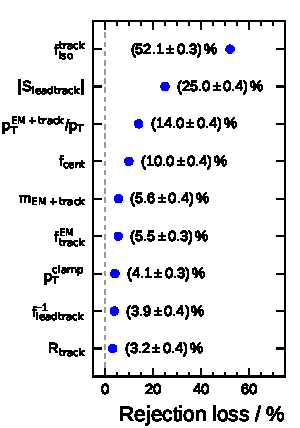
\includegraphics{./figures/bdt_perf/var_importance/1p_iter2.pdf}
    \subcaption{Iteration 2}
  \end{subfigure}
  \caption{Variable importance (1-prong). Averaged rejection loss over a
    gamma-tautau like dijet spectrum. Tight working point.}
  \label{fig:variable_importance_1p_app}
\end{figure}

\begin{figure}[htb]
  \centering
  \begin{subfigure}[t]{0.32\textwidth}
    \centering
    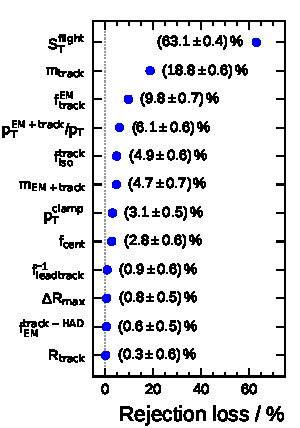
\includegraphics{./figures/bdt_perf/var_importance/3p_iter1.pdf}
    \subcaption{Iteration 1}
  \end{subfigure}
  \begin{subfigure}[t]{0.32\textwidth}
    \centering
    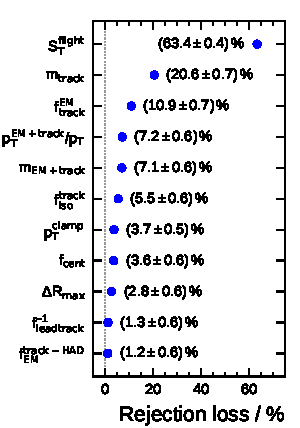
\includegraphics{./figures/bdt_perf/var_importance/3p_iter2.pdf}
    \subcaption{Iteration 2}
  \end{subfigure}
  \begin{subfigure}[t]{0.32\textwidth}
    \centering
    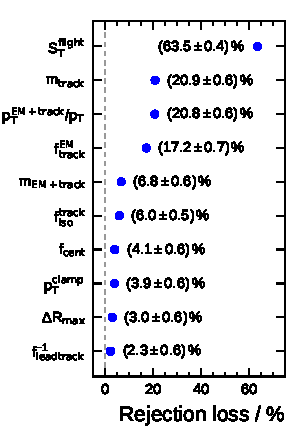
\includegraphics{./figures/bdt_perf/var_importance/3p_iter3.pdf}
    \subcaption{Iteration 3}
  \end{subfigure}

  \caption{Variable importance (3-prong). Averaged rejection loss over a
    gamma-tautau like dijet spectrum. Tight working point.}
  \label{fig:variable_importance_3p_app}
\end{figure}

\clearpage
\section{Post-Optimisation Working Points}
\label{app:bdt_working_point_rejection}

\begin{figure}[htb]
  \centering
  \begin{subfigure}{0.48\textwidth}
    \centering
    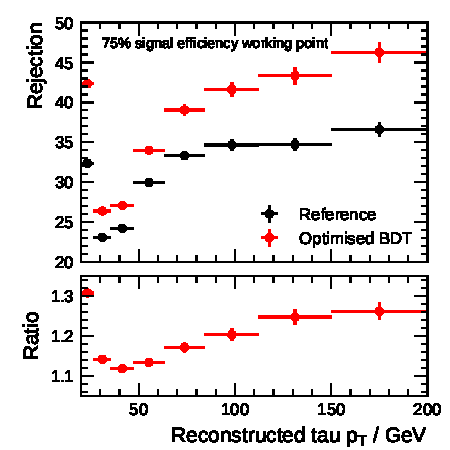
\includegraphics{./figures/bdt_perf/post_optimisation/rejection_medium_1p.pdf}
    \subcaption{medium}
  \end{subfigure}\hfill
  \begin{subfigure}{0.48\textwidth}
    \centering
    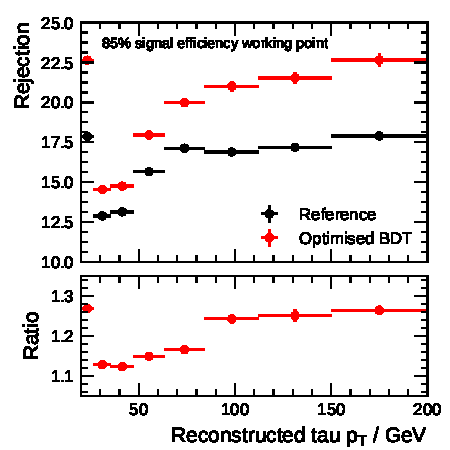
\includegraphics{./figures/bdt_perf/post_optimisation/rejection_loose_1p.pdf}
    \subcaption{loose}
  \end{subfigure}
  \caption{1-prong}
\end{figure}

\begin{figure}[htb]
  \centering
  \begin{subfigure}{0.48\textwidth}
    \centering
    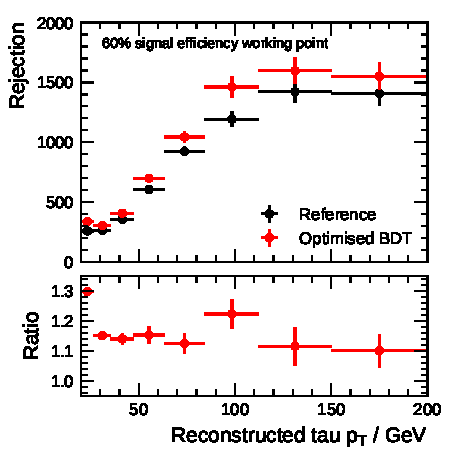
\includegraphics{./figures/bdt_perf/post_optimisation/rejection_medium_3p.pdf}
    \subcaption{medium}
  \end{subfigure}\hfill
  \begin{subfigure}{0.48\textwidth}
    \centering
    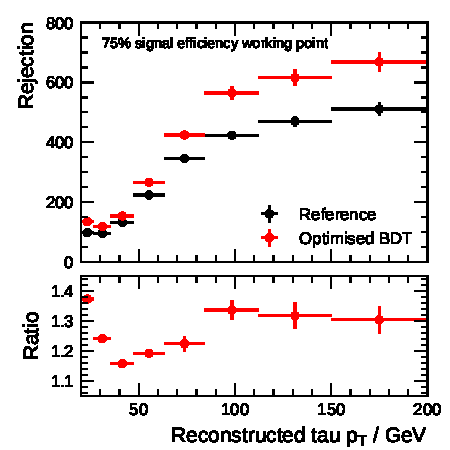
\includegraphics{./figures/bdt_perf/post_optimisation/rejection_loose_3p.pdf}
    \subcaption{loose}
  \end{subfigure}
  \caption{3-prong}
\end{figure}


\begin{figure}[htb]
  \centering
  \begin{subfigure}{0.48\textwidth}
    \centering
    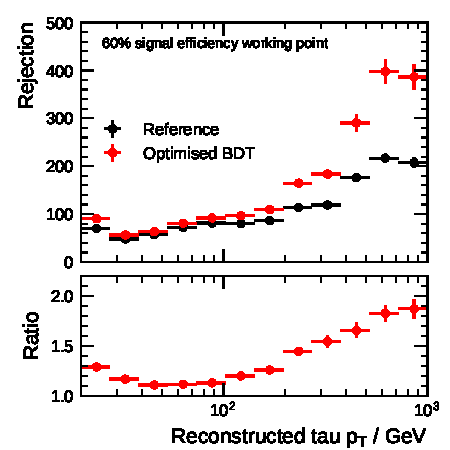
\includegraphics{./figures/bdt_perf/post_optimisation/1p_highpt/rejection_tight_ratio_highpt.pdf}
    \subcaption{tight}
  \end{subfigure}\hfill
  \begin{subfigure}{0.48\textwidth}
    \centering
    \includegraphics{./figures/bdt_perf/post_optimisation/1p_highpt/rejection_medium_ratio_highpt.pdf}
    \subcaption{medium}
  \end{subfigure}
  \begin{subfigure}{0.48\textwidth}
    \centering
    \includegraphics{./figures/bdt_perf/post_optimisation/1p_highpt/rejection_loose_ratio_highpt.pdf}
    \subcaption{loose}
  \end{subfigure}
  \caption{1-prong high-pt}
\end{figure}

\begin{figure}[htb]
  \centering
  \begin{subfigure}{0.48\textwidth}
    \centering
    \includegraphics{./figures/bdt_perf/post_optimisation/3p_highpt/rejection_tight_ratio_highpt.pdf}
    \subcaption{tight}
  \end{subfigure}\hfill
  \begin{subfigure}{0.48\textwidth}
    \centering
    \includegraphics{./figures/bdt_perf/post_optimisation/3p_highpt/rejection_medium_ratio_highpt.pdf}
    \subcaption{medium}
  \end{subfigure}
  \begin{subfigure}{0.48\textwidth}
    \centering
    \includegraphics{./figures/bdt_perf/post_optimisation/3p_highpt/rejection_loose_ratio_highpt.pdf}
    \subcaption{loose}
  \end{subfigure}
  \caption{3-prong high-pt}
\end{figure}


\clearpage
\section{Rejection vs.\ Initiating Parton}
\begin{figure}[htb]
  \centering
  \begin{subfigure}[t]{0.48\textwidth}
    \centering
    \includegraphics{./figures/bdt_perf/parton/truth_parton_1p.pdf}
    \caption{1-prong}
  \end{subfigure}\hfill
  \begin{subfigure}[t]{0.48\textwidth}
    \centering
    \includegraphics{./figures/bdt_perf/parton/truth_parton_3p.pdf}
    \caption{3-prong. Loose working point (Tight has too much rejection for
      limited stats)}
  \end{subfigure}
  \caption{Rejection vs initiating parton}
\end{figure}

\todo[inline]{Due to the longer decay chain of B-hadrons, the number of
  particles and angular spread is larger for a b-jet than a light-quark jet.}

\clearpage
\section{Decay Mode Classification Experiments}
\label{sec:app_decay_mode_exp}
\begin{figure}[htb]
  \begin{subfigure}[t]{0.48\textwidth}
    \centering
    \includegraphics{./figures/decay_mode_classification/experiments/mig_mat_conversions.pdf}
    \subcaption{Migration matrix}
  \end{subfigure}\hfill
  \begin{subfigure}[t]{0.48\textwidth}
    \centering
    \includegraphics{./figures/decay_mode_classification/experiments/comp_mat_conversions.pdf}
    \subcaption{Composition matrix}
  \end{subfigure}
  \caption{Conversion tracks}
\end{figure}

\begin{figure}[htb]
  \begin{subfigure}[t]{0.48\textwidth}
    \centering
    \includegraphics{./figures/decay_mode_classification/experiments/mig_mat_shots.pdf}
    \subcaption{Migration matrix}
  \end{subfigure}\hfill
  \begin{subfigure}[t]{0.48\textwidth}
    \centering
    \includegraphics{./figures/decay_mode_classification/experiments/comp_mat_shots.pdf}
    \subcaption{Composition matrix}
  \end{subfigure}
  \caption{Shots}
\end{figure}

\begin{figure}[htb]
  \begin{subfigure}[t]{0.48\textwidth}
    \centering
    \includegraphics{./figures/decay_mode_classification/experiments/mig_mat_moments.pdf}
    \subcaption{Migration matrix}
  \end{subfigure}\hfill
  \begin{subfigure}[t]{0.48\textwidth}
    \centering
    \includegraphics{./figures/decay_mode_classification/experiments/comp_mat_moments.pdf}
    \subcaption{Composition matrix}
  \end{subfigure}
  \caption{Add.\ cluster moments}
\end{figure}

\begin{figure}[htb]
  \begin{subfigure}[t]{0.48\textwidth}
    \centering
    \includegraphics{./figures/decay_mode_classification/experiments/mig_mat_hadronic_pfos.pdf}
    \subcaption{Migration matrix}
  \end{subfigure}\hfill
  \begin{subfigure}[t]{0.48\textwidth}
    \centering
    \includegraphics{./figures/decay_mode_classification/experiments/comp_mat_hadronic_pfos.pdf}
    \subcaption{Composition matrix}
  \end{subfigure}
  \caption{Hadronic PFOs}
\end{figure}

\begin{figure}[htb]
  \begin{subfigure}[t]{0.48\textwidth}
    \centering
    \includegraphics{./figures/decay_mode_classification/experiments/mig_mat_sub_e_2.pdf}
    \subcaption{Migration matrix}
  \end{subfigure}\hfill
  \begin{subfigure}[t]{0.48\textwidth}
    \centering
    \includegraphics{./figures/decay_mode_classification/experiments/comp_mat_sub_e_2.pdf}
    \subcaption{Composition matrix}
  \end{subfigure}
  \caption{$p_\text{T}$-fraction}
\end{figure}

\clearpage
\section{Combined After Tau-ID}

\begin{figure}[htbp]
  \begin{subfigure}{0.48\textwidth}
    \centering
    \includegraphics{./figures/decay_mode_classification/combined_sub_e_moments_shots_conv_ptcut_1_5/mig_mat_med_id.pdf}
    \subcaption{Migration matrix}
  \end{subfigure}\hfill
  \begin{subfigure}{0.48\textwidth}
    \centering
    \includegraphics{./figures/decay_mode_classification/combined_sub_e_moments_shots_conv_ptcut_1_5/comp_mat_med_id.pdf}
    \subcaption{ Purity matrix}
  \end{subfigure}
  \caption{Combined with medium tau id}
  \label{fig:decay_mode_combined_med_id}
\end{figure}

\clearpage
\section{Track-Constrained Decay Mode Classification}
\label{app:mode_classification_track_constraint}

\begin{figure}[htbp]
  \begin{subfigure}{0.48\textwidth}
    \centering
    \includegraphics{./figures/decay_mode_classification/combined_sub_e_moments_shots_conv_ptcut_1_5/mig_mat.pdf}
    \subcaption{Extended model without track constraint.}
  \end{subfigure}\hfill
  \begin{subfigure}{0.48\textwidth}
    \centering
    \includegraphics{./figures/decay_mode_classification/combined_sub_e_moments_shots_conv_ptcut_1_5/mig_mat_use_ntracks.pdf}
    \subcaption{Extended model with track constraint.}
  \end{subfigure}
  \caption{Migration matrix for the extended model including conversion, shot
    and additional cluster information. The model is constrained by setting
    estimated mode probabilities to zero for modes not consistent with the
    number of reconstructed tracks.}
\end{figure}

\clearpage
\section{High-$p_\text{T}$}
\label{sec:combined_high_pt_migration}

\begin{figure}[htb]
    \begin{subfigure}{0.48\textwidth}
    \centering
    \includegraphics{./figures/decay_mode_classification/highpt/mig_mat_pt_less_100.pdf}
    \subcaption{Migration matrix. $p_\text{T} < \SI{100}{\giga\electronvolt}$}
  \end{subfigure}\hfill
  \begin{subfigure}{0.48\textwidth}
    \centering
    \includegraphics{./figures/decay_mode_classification/highpt/comp_mat_pt_less_100.pdf}
    \subcaption{Migration matrix. $p_\text{T} < \SI{100}{\giga\electronvolt}$}
  \end{subfigure}
  \begin{subfigure}{0.48\textwidth}
    \centering
    \includegraphics{./figures/decay_mode_classification/highpt/mig_mat_pt_geq_100.pdf}
    \subcaption{Migration matrix. $p_\text{T} > \SI{100}{\giga\electronvolt}$}
  \end{subfigure}\hfill
  \begin{subfigure}{0.48\textwidth}
    \centering
    \includegraphics{./figures/decay_mode_classification/highpt/comp_mat_geq_100.pdf}
    \subcaption{Purity matrix. $p_\text{T} > \SI{100}{\giga\electronvolt}$}
  \end{subfigure}
  \caption{highpt}
  \label{fig:highpt_matrices}
\end{figure}

\clearpage
\section{TODOS}
\listoftodos

%%% Local Variables:
%%% mode: latex
%%% TeX-master: "mythesis"
%%% End:
